\section{Experimentos}
	%Todos los experimentos se repitieron 20 veces. Para reproducirlos se debe ejecutar exp/exp.sh -n 20  
	
	\subsection{Experimento 1}
		En el primer experimento se genera una determinada cantidad de imágenes tomando una imagen grande y cambiando su tamaño disminuyendo sus dimensiones.
	
		Luego, se ejecuta el filtro Blur con cada una de las imágenes y se compara el tiempo de ejecución de las implementaciones en C y assembler.
	
		Esto se repite para el filtro Diff, con la diferencia de que para cada tamaño de imágen se generan dos imágenes con ciertas modificaciones para poder observar el buen funcionamiento del mismo.


	\subsubsection{Hipótesis} 
		El resultado esperado es que la implementación en assembler de ambos filtros sea más eficiente, sin importar el tamaño de la imagen. Esto sucede ya que a diferencia de C, assembler utiliza SIMD para procesar píxeles, por lo tanto es posible trabajar con 4 píxeles en simultaneo.

	\subsubsection{Valores utilizados como parámetros} 		
		En este experimento el ancho de las imágenes utilizadas como parámetro se encuentran en un rango entre 24 y 1800 píxeles.Además, para el filtro Blur se utilizó $Radio = 15$ y $Sigma = 5$.

	\subsubsection{Resultados}
   	{\centering \begin{tabular}{c}
      {\small Filtro Diferencia} \\
      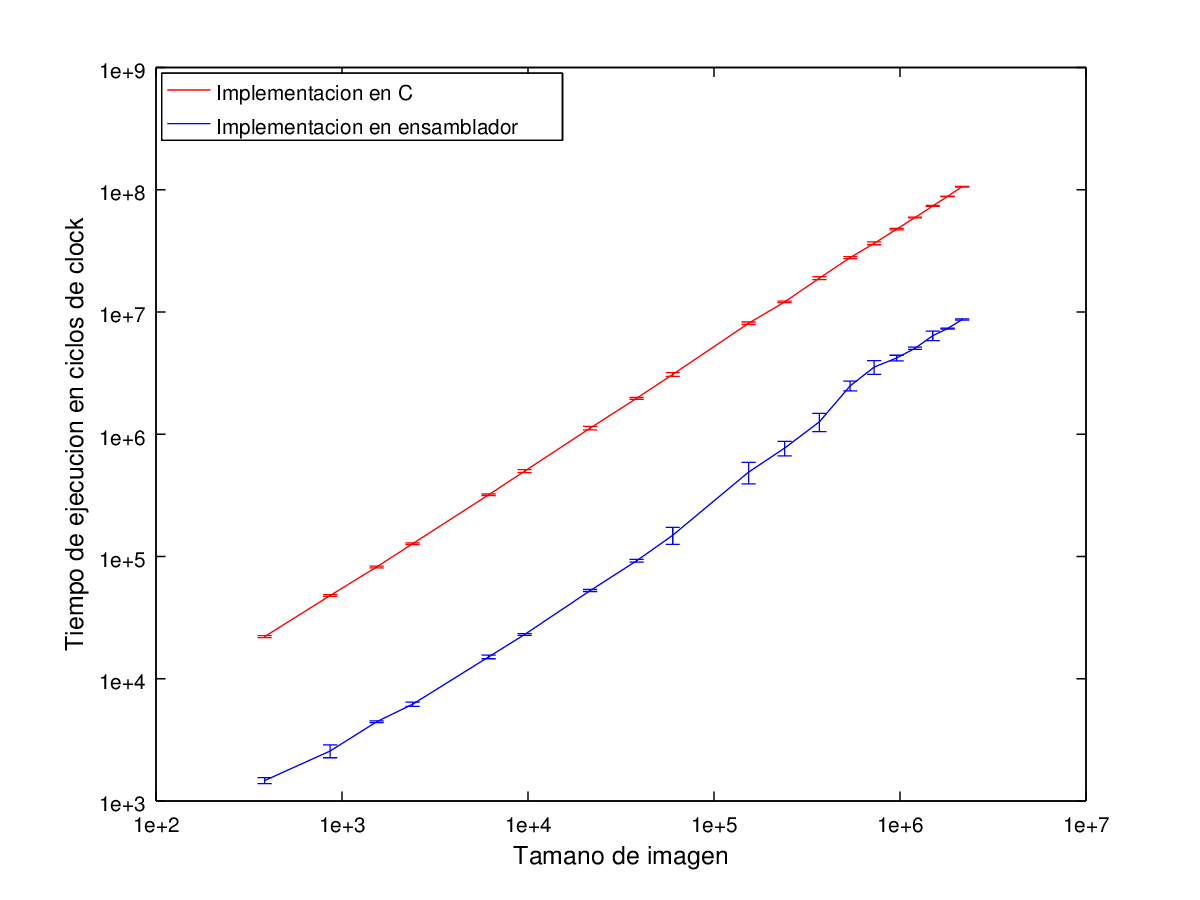
\includegraphics[width=12cm]{../exp/graficos/exp1-diff-c_vs_asm.png} \\
    \end{tabular}}

    {\centering \begin{tabular}{c}
      {\small Filtro Diferencia - Tiempo de ejecución normalizado por píxel} \\
      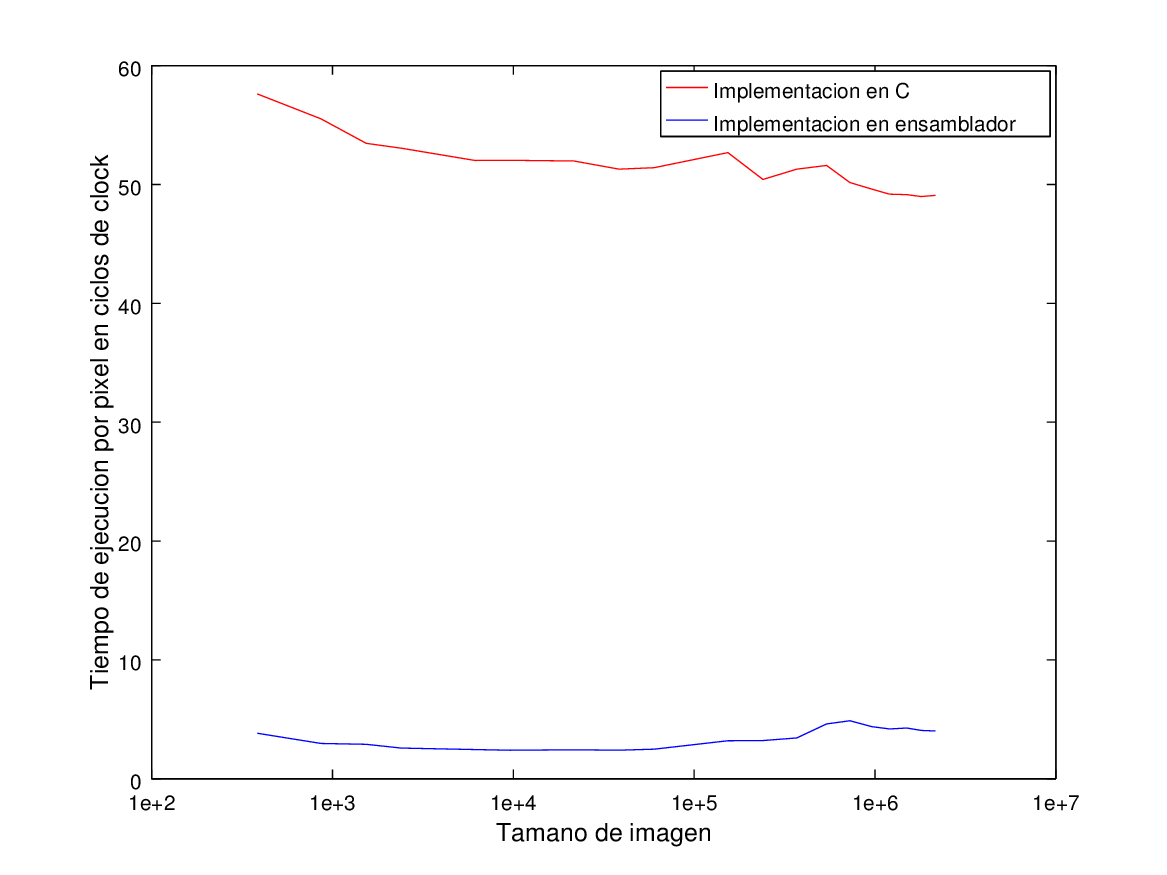
\includegraphics[width=12cm]{../exp/graficos/exp1-diff-tiempo_por_pixel.png} \\
    \end{tabular}}

	{\centering \begin{tabular}{c}
      {\small Filtro Blur} \\
      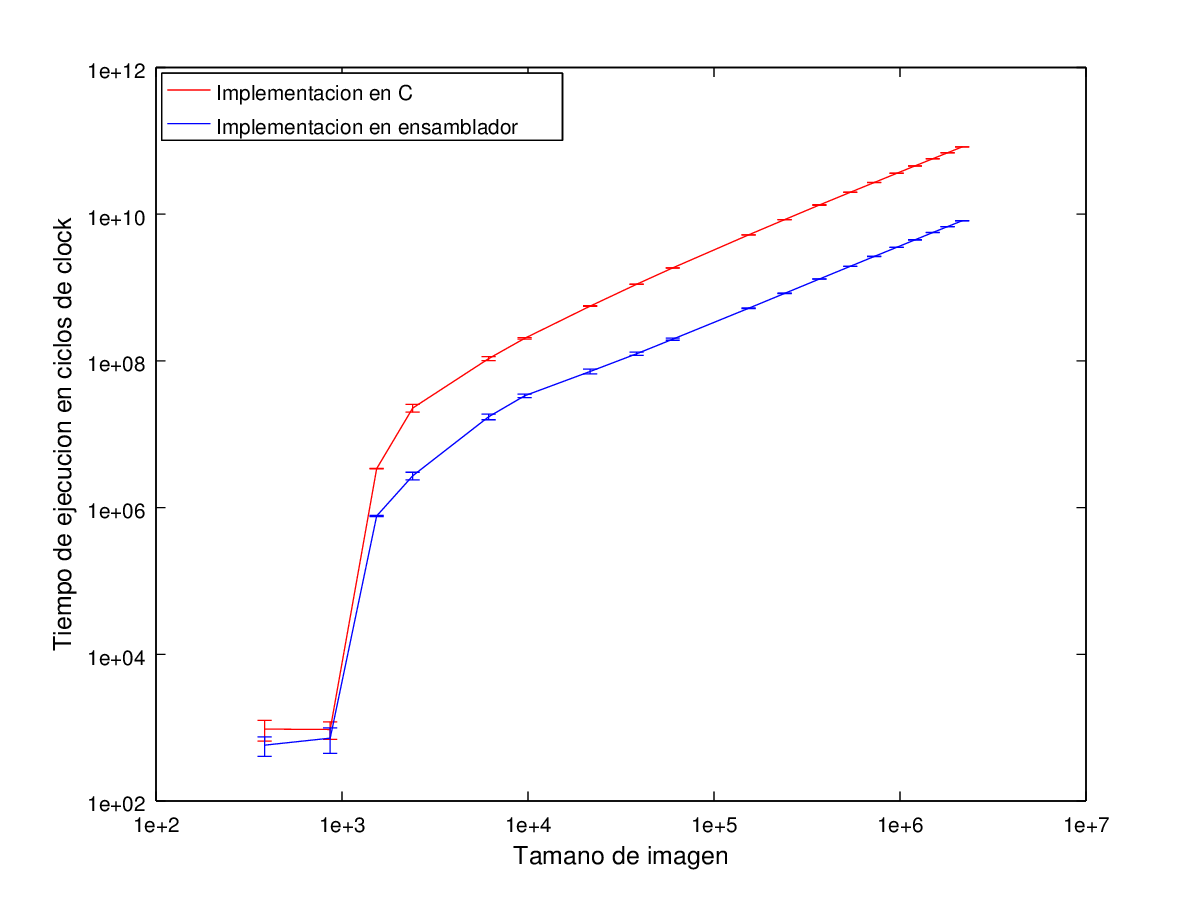
\includegraphics[width=12cm]{../exp/graficos/exp1-blur-c_vs_asm.png} \\
    \end{tabular}}

   	{\centering \begin{tabular}{c}
      {\small Filtro Blur - Tiempo de ejecución normalizado por píxel} \\
      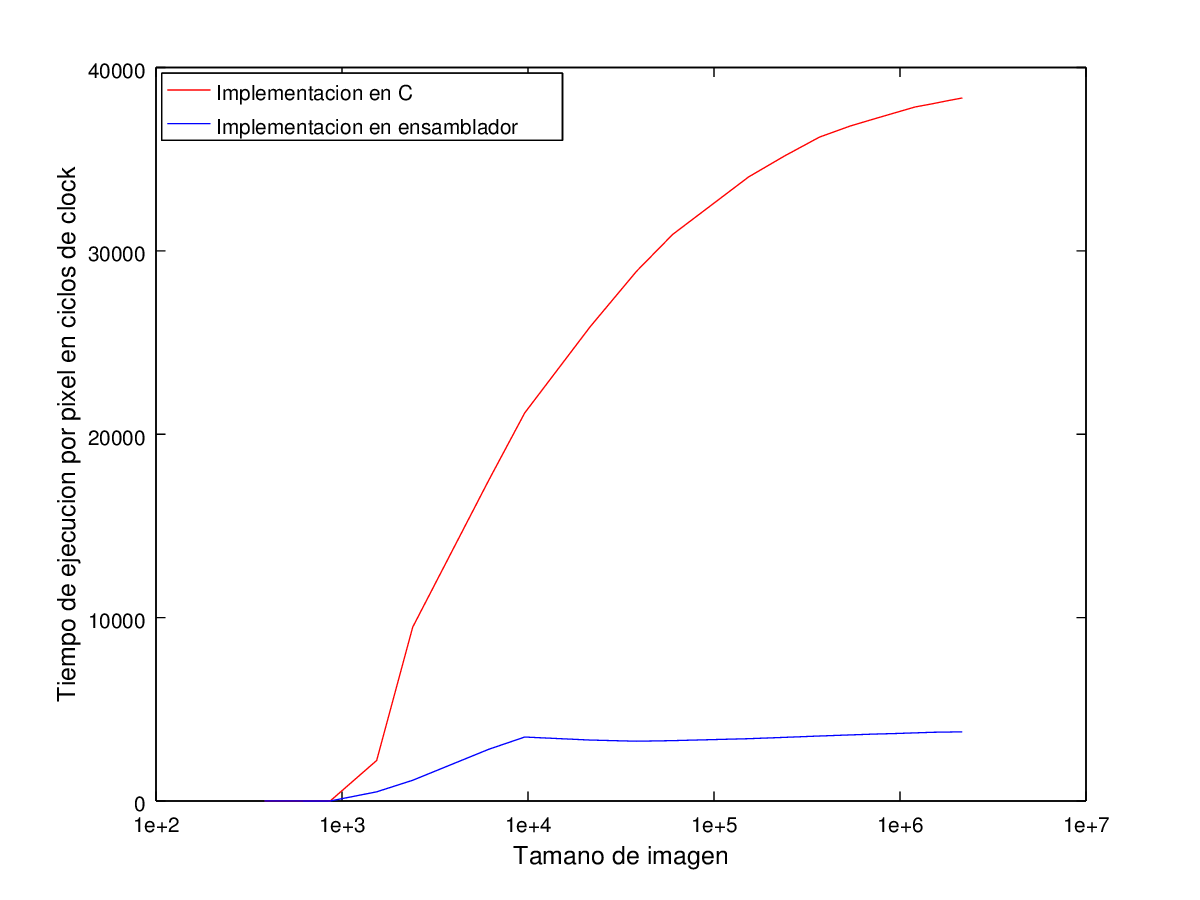
\includegraphics[width=12cm]{../exp/graficos/exp1-blur-tiempo_por_pixel.png} \\
    \end{tabular}}


	\subsubsection{Conclusión} 
		Como se observa en los resultados, la implementación en assembler es más rápida que la implementación en C para todos los tamaños de imagen. Esto se debe a que la primera utiliza SIMD para procesar los píxeles mientras que la segunda no. Lo pudimos comprobar desensamblando el archivo objeto y examinando el código. 


	\subsection{Experimento 2}
		El objetivo de este experimento es observar como se afecta la eficiencia del algoritmo Blur, en cada una de las implementaciones al tomar siempre la misma imagen pero variando el radio.
	
		De esta forma, podemos ver la diferencia de tiempo de ejecución para distintos valores de este parámetro, tanto para la implementación en C como la de assembler. Este experimento lo vamos a realizar normalizando el resultado, para considerar el tiempo de procesamiento por píxel.

		\subsubsection{Hipótesis} 
			Suponemos que a medida que el valor del radio sea mayor, el tiempo de ejecución en las dos implementaciones aumenta. Esto se debe a que el tamaño de la matriz de convolución y de la submatriz imagen es $(2 \times \mathtt{radio} + 1) \times (2 \times \mathtt{radio} + 1) \times 4$. 

		\subsubsection{Valores utilizados como parámetros} 
		La dimensión de la imagen utilizada es 400 filas y 600 columnas. El valor del sigma es 5 y los radios toman valores entre 1 y 40.

		\subsubsection{Resultados}

		{\centering \begin{tabular}{c}
      		{\small Filtro Blur - Tiempo de ejecución según radio} \\
      		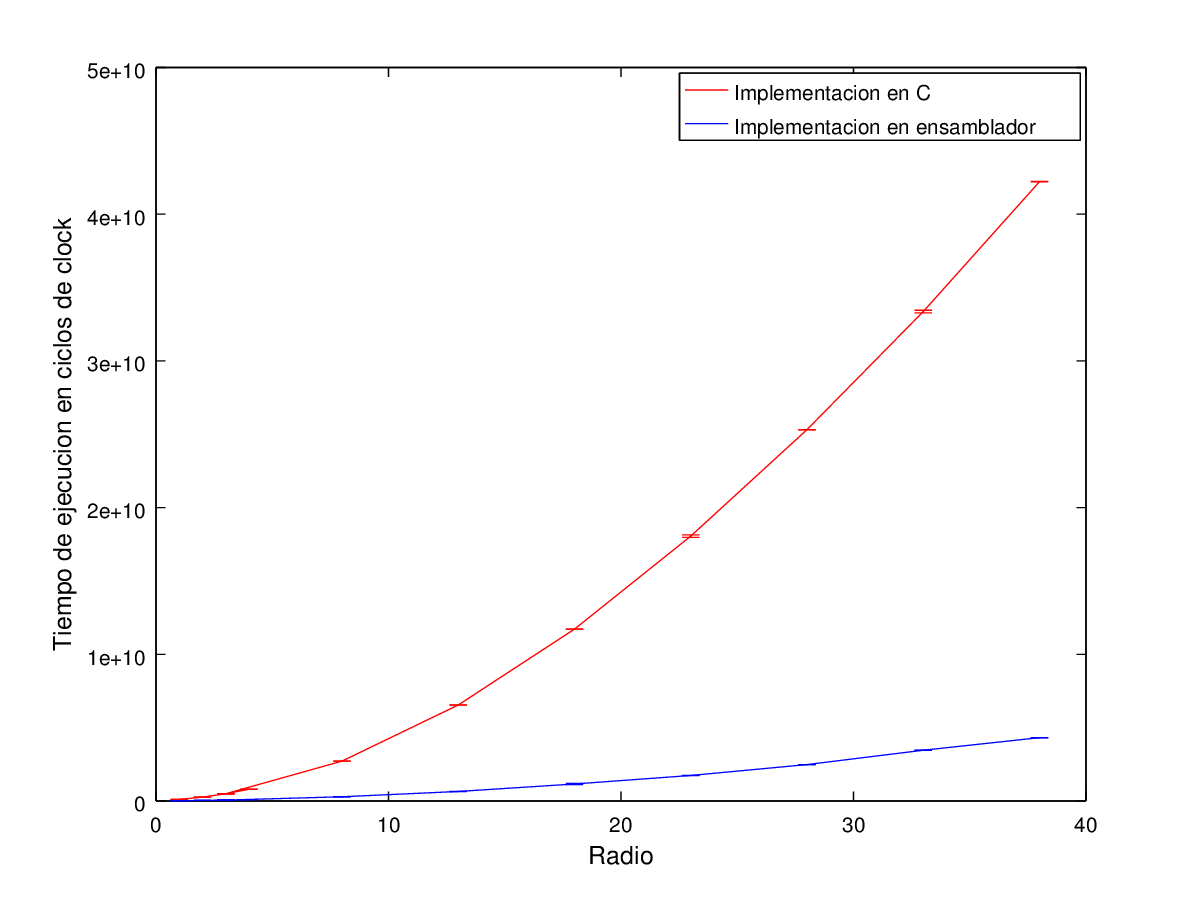
\includegraphics[width=12cm]{../exp/graficos/exp2-tiempo_segun_radio.png} \\
    	\end{tabular}}

		\subsubsection{Conclusión}
			Podemos observar en los gráficos que a medida que los radios aumentan, también lo hace el tiempo de ejecución. Por lo tanto, pudimos comprobar nuestra hipótesis. Esto sucede ya que cuanto mayor es el tamaño de la matriz de convolución, crece la cantidad de iteraciones que se realiza por cada píxel.

			


	\subsection{Experimento 3}
		Este experimento es similar al anterior, también se realiza sobre las dos implementaciones del filtro Blur y se considera siempre la misma imagen. En este caso el radio se mantiene constante pero el valor del sigma se modifica. También se va a utilizar el resultado normalizado, para poder estudiar el tiempo de procesamiento por píxel. 

		\subsubsection{Hipótesis} 
			Debido a que el valor del sigma es utilizado solamente para realizar un cálculo por cada posición de la matriz de convolución, suponemos que modificar este valor no alterará el tiempo de ejecución.

		\subsubsection{Valores utilizados como parámetros} 
		La dimensión de la imagen utilizada es 400 filas y 600 columnas. El valor del radio es 10 y sigma toma valores entre 0.5 y 50.

		\subsubsection{Resultados}

		{\centering \begin{tabular}{c}
      		{\small Filtro Blur - Tiempo de ejecución según sigma} \\
      		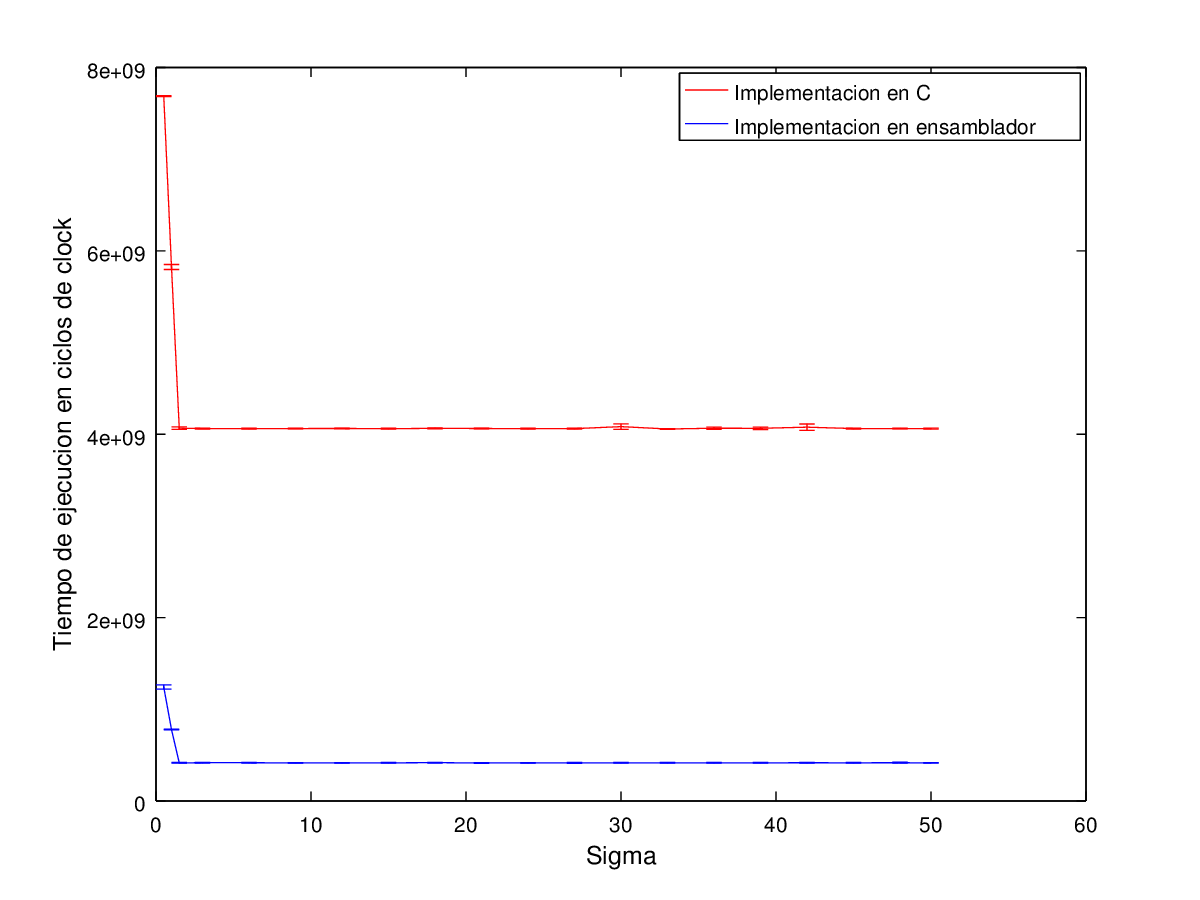
\includegraphics[width=12cm]{../exp/graficos/exp3-tiempo_segun_sigma.png} \\
    	\end{tabular}}

		\subsubsection{Conclusión}


	\subsection{Experimento 4}
		Otras de las pruebas consiste en comparar los tiempos de ejecución de diferentes implementaciones de los filtros en assembler. Nos interesa medir el peso que tienen en el tiempo de ejecución los llamados a funciones auxiliares. Para esto, queremos comparar el rendimiento de una implementación que utiliza llamados a estas funciones, con el de otra que tiene todas las instrucciones necesarias en el mismo bloque de código (sin utilizar esas funciones auxiliares). 
		
		Este experimento se realiza una determinada cantidad de veces con distintos tamaños de imagen.

		\subsubsection{Hipótesis} 
			Creemos que la versión del código implementada en assembler que no realiza llamados a funciones va a tener un mejor rendimiento, ya que se evita el overhead que producen estos llamados.
		
		\subsubsection{Valores utilizados como parámetros} 
			En este experimento el ancho de las imágenes utilizadas como parámetro se encuentran en un rango entre 24 y 1800 píxeles.Además, para el filtro Blur se utilizó $Radio = 15$ y $Sigma = 5$.


		\subsubsection{Resultados}
		{\centering \begin{tabular}{c}
      		{\small Filtro Diferencia} \\
      		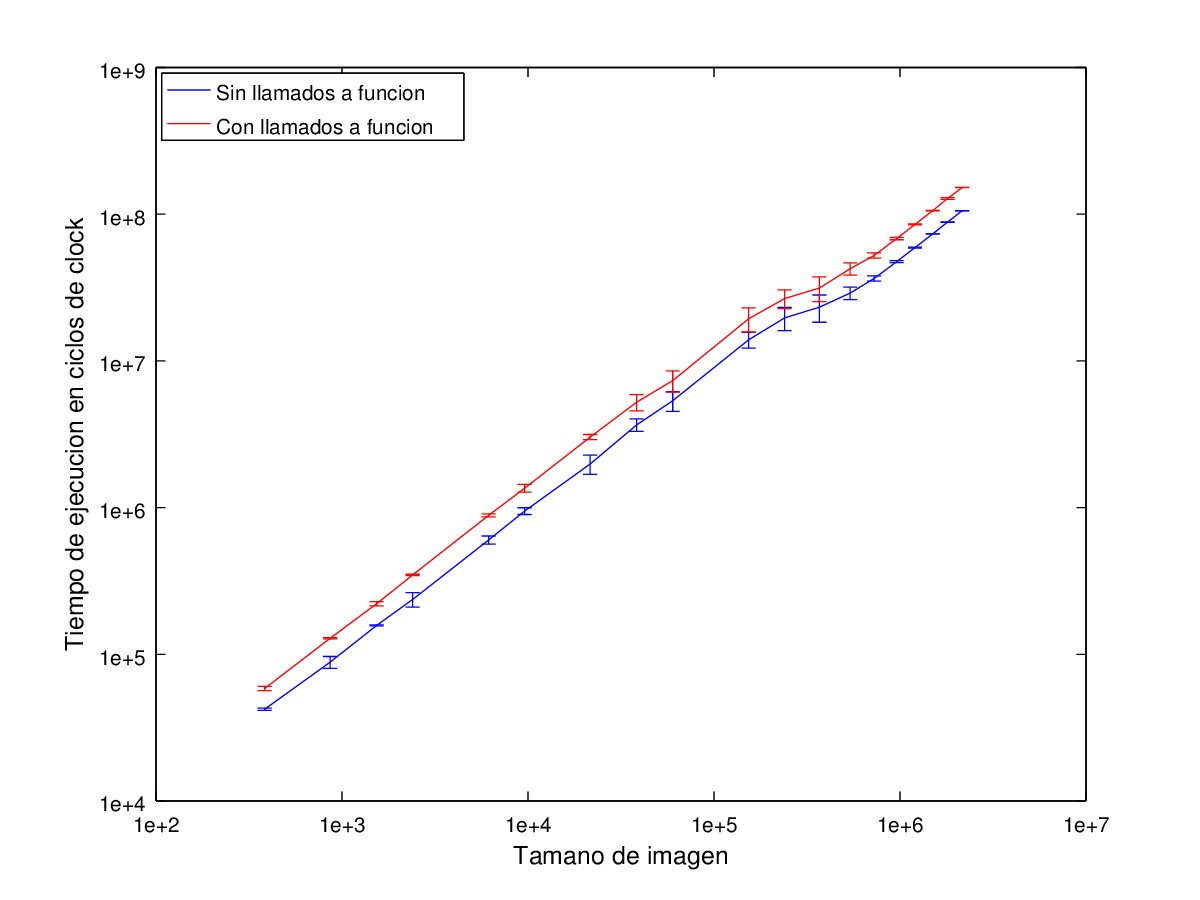
\includegraphics[width=12cm]{../exp/graficos/exp4-diff-c_vs_c2.png} \\
    	\end{tabular}}

		{\centering \begin{tabular}{c}
      		{\small Filtro Blur} \\
      		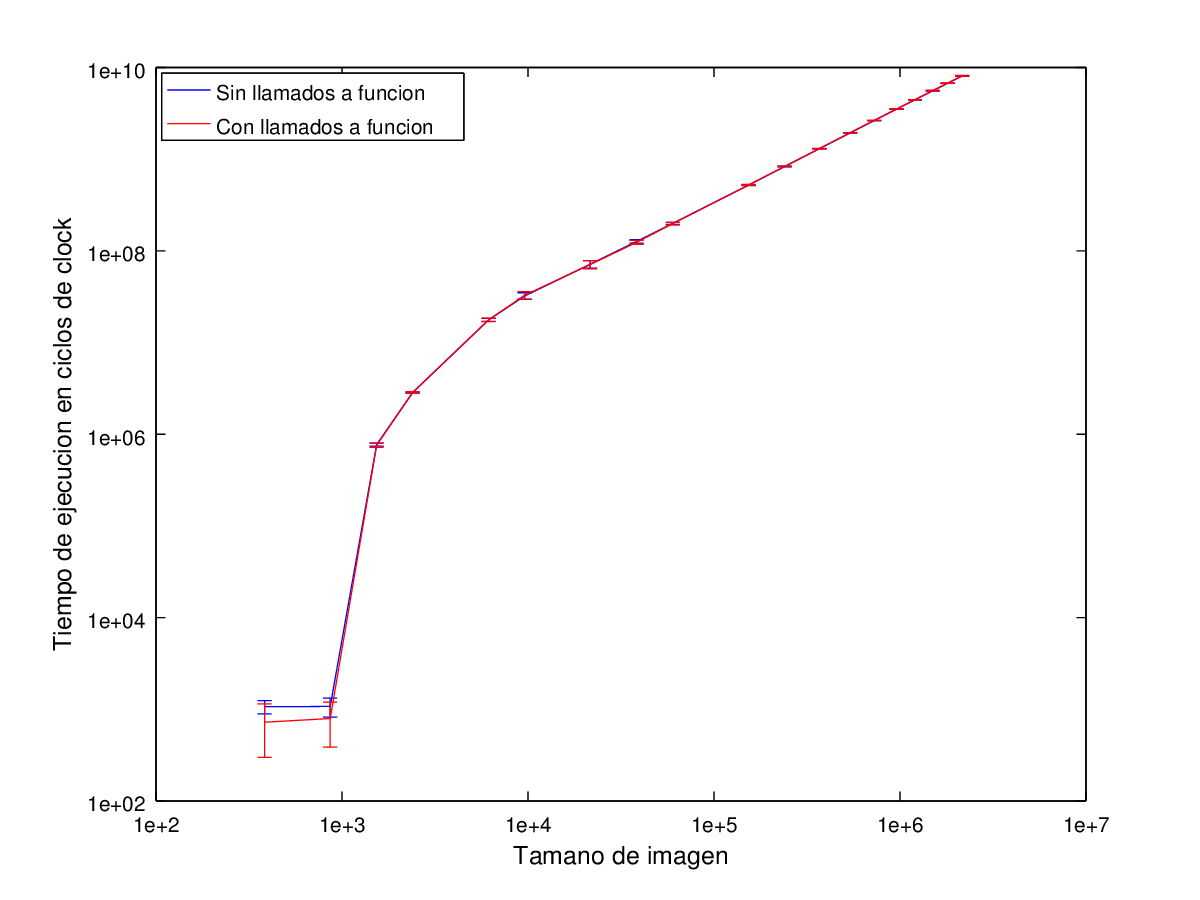
\includegraphics[width=12cm]{../exp/graficos/exp4-blur-asm_vs_asm2.png} \\
    	\end{tabular}}

		\subsubsection{Conclusión}		